% --------------------------------------------------------------
% This is all preamble stuff that you don't have to worry about.
% Head down to where it says "Start here"
% --------------------------------------------------------------
 
\documentclass[11pt]{article}
 
\usepackage[margin=0.5in]{geometry} 
\usepackage{amsmath,amsthm,amssymb, enumerate, soul, float, multirow, varwidth, bm, hyperref}
\usepackage[hashEnumerators,smartEllipses]{markdown}
\usepackage{graphicx}
\usepackage[ruled,vlined]{algorithm2e}
\graphicspath{ {./images/} }
 
\begin{document}

% --------------------------------------------------------------
%                         Start here
% --------------------------------------------------------------
 
\title{Repository Analysis Report for Netron}
\author{Pengnan Fan \\ pengnan.fan@mail.mcgill.ca}

\maketitle

\section{Introduction}
In this report, I investigated an open source project (\href{https://github.com/openstack/neutron}{openstack/netron}) from GitHub and studied module-level file changes of its master branch in the past six month. For the study, two questions are focused:
\begin{enumerate}
    \item{
        What are the top-12 most frequent changed modules?
    }
    \item{
        How many commits occurred in the past six month?
    }
    \item{
        How much line changes (addition and deletion) occurred in the past six month? 
    }
\end{enumerate}
For this report, commit records are collected through GitHub API and visualized by a python script.

\section{Result}
According to my script, there are \textbf{472 commits} occurred in the past six month. These commits include at least one file change under the \textit{/neutron} directory of the studied project. These commits have \textbf{40987 line changes} in total, where \textbf{35204} of them are \textbf{additions} and \textbf{13883} are \textbf{deletions}.
\begin{table}[H]
    \centering
    \begin{tabular}{|c|c|c|c|}
         \hline
         module & total & add & total \\
         \hline
         test & 25394 &18394 & 7000\\
         plugins & 6539 & 4265 & 2274\\
         db & 5679 & 4050 & 1629\\
         agent & 3763 & 2886 & 877\\
         services & 2720 & 1748 & 972\\
         extensions & 949 & 897 & 52\\
         objects & 935 & 722 & 213\\
         cmd & 933 & 929 & 4\\
         quota & 560 & 178 & 382\\
         common & 486 & 338 & 148\\
         conf & 469 & 390 & 79\\
         api & 385 & 234 & 151\\
         \hline
    \end{tabular}
    \caption{Details for Top-12 Most Frequent Modified Modules under /neutron}
    \label{tab:1}
\end{table}
And the top-12 most frequent modified modules are listed in table\ref{tab:1}. 
In addition, I also visualized the portion of addition and deletion for the 12 modules. From the charts, it is observed that tests, plugins and db are the top-3 most frequent addition/deletion modules.
\begin{figure}[H]
    \centering
    \includegraphics[width=0.5\linewidth]{./img/odification.png}
    \caption{Top-12 Most Frequent Modified Modules under /neutron}
    \label{fig:1}
\end{figure}
\begin{figure}[H]
    \centering
    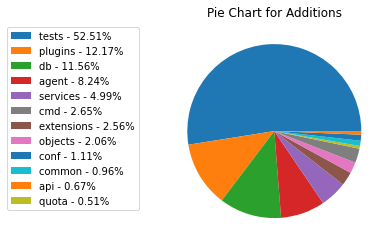
\includegraphics[width=0.5\linewidth]{./img/addition_pie.png}
    \caption{Pie Chart for Addition of the Top-12 Modules}
    \label{fig:2}
\end{figure}
\begin{figure}[H]
    \centering
    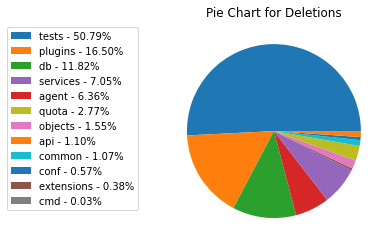
\includegraphics[width=0.5\linewidth]{./img/deletion_pie.png}
    \caption{Pie Chart for Deletion of the Top-12 Modules}
    \label{fig:3}
\end{figure}


\end{document}